% Sparse-Koopman multibasin paper — single-page overview diagram.
% Standalone TikZ; compile with: pdflatex paper_overview_diagram.tex
%
% Three-panel storyline (Problem -> Model -> Idea), no experiments/results.
% Designed to be visually consistent with the paper (Computer Modern serif,
% LaTeX math typesetting, vector graphics).

\documentclass[tikz,border=8pt]{standalone}

\usepackage[T1]{fontenc}
\usepackage{amsmath,amssymb}
\usepackage{xcolor}
\usepackage{tikz}
\usetikzlibrary{positioning,arrows.meta,shapes.misc,calc,fit,backgrounds}

% --- palette ---------------------------------------------------------------
\definecolor{bgsoft}{HTML}{F7F6F1}
\definecolor{cardborder}{HTML}{D8D9D4}
\definecolor{textdark}{HTML}{1E2761}
\definecolor{textbody}{HTML}{1F2937}
\definecolor{textmuted}{HTML}{6B7280}
\definecolor{cellinactive}{HTML}{ECECE5}
\definecolor{cellinactivebd}{HTML}{C6C6BF}
\definecolor{basinA}{HTML}{6B5B95}   % purple
\definecolor{basinB}{HTML}{178582}   % teal
\definecolor{basinC}{HTML}{D9755C}   % coral
\definecolor{ideabg}{HTML}{FFF6D6}
\definecolor{ideabd}{HTML}{E2C97A}
\definecolor{okgreen}{HTML}{2E7D32}
\definecolor{badred}{HTML}{B23A48}
\definecolor{cardbg}{HTML}{FFFFFF}

% --- TikZ styles -----------------------------------------------------------
\tikzset{
  paneltag/.style={font=\fontsize{8.5}{10}\selectfont\bfseries\sffamily,
                   text=#1},
  paneltitle/.style={font=\fontsize{12}{14}\selectfont\bfseries,
                     text=textdark,align=left,inner sep=0pt},
  body/.style={font=\fontsize{10}{12.5}\selectfont,text=textbody,align=left,
               inner sep=0pt},
  bodysmall/.style={font=\fontsize{9}{11}\selectfont,text=textbody,
                    align=left,inner sep=0pt},
  caption/.style={font=\fontsize{8.5}{10}\selectfont\itshape,text=textmuted,
                  align=center,inner sep=0pt},
  pipebox/.style={draw=cardborder,line width=0.5pt,fill=bgsoft,
                  rounded corners=1.6pt,inner xsep=4pt,inner ysep=3.5pt,
                  font=\fontsize{10}{12}\selectfont,text=textdark,
                  align=center},
  arr/.style={-{Stealth[length=4.5pt]},line width=0.6pt,color=textmuted},
  arrK/.style={-{Stealth[length=5pt]},line width=0.8pt,color=textdark},
  cell/.style={draw=cellinactivebd,fill=cellinactive,line width=0.3pt,
               minimum width=4mm,minimum height=6.5mm,inner sep=0pt},
  acell/.style={draw=#1,fill=#1,line width=0.3pt,
                minimum width=4mm,minimum height=6.5mm,inner sep=0pt},
  ccell/.style={draw=cellinactivebd,fill=cellinactive,line width=0.3pt,
                minimum width=3.6mm,minimum height=6mm,inner sep=0pt},
  acell2/.style={draw=#1,fill=#1,line width=0.3pt,
                 minimum width=3.6mm,minimum height=6mm,inner sep=0pt},
  basinbadge/.style={draw=#1,fill=#1!12,line width=0.5pt,rounded corners=2pt,
                     inner xsep=4pt,inner ysep=3pt,
                     font=\fontsize{9.5}{11}\selectfont\bfseries,text=#1,
                     minimum width=11mm,align=center},
  seqbox/.style={draw=cardborder,fill=bgsoft,line width=0.4pt,
                 rounded corners=1.5pt,inner xsep=4pt,inner ysep=2.5pt,
                 font=\fontsize{9}{10.5}\selectfont,text=textdark,
                 align=center,minimum height=6mm},
  seqcolor/.style={draw=#1,fill=#1,line width=0.4pt,rounded corners=1.5pt,
                   inner xsep=5pt,inner ysep=2.5pt,
                   font=\fontsize{9}{10.5}\selectfont\bfseries,text=white,
                   align=center,minimum height=6mm},
}

% --- helper: draw a "basin" — colored well + center dot + inward arrows ----
\newcommand{\drawbasin}[4]{% (#1=cx in cm, #2=cy in cm, #3=color, #4=label)
  \begin{scope}[shift={(#1,#2)}]
    \fill[#3,opacity=0.18] (0,0) circle (8mm);
    \fill[#3,opacity=0.30] (0,0) circle (5mm);
    \fill[#3]              (0,0) circle (1.4mm);
    \foreach \a in {35,125,215,305}{%
      \draw[-{Stealth[length=2pt]},#3,line width=0.45pt]
        (\a:6mm) -- (\a:3mm);
    }
    \node[font=\fontsize{8.5}{10}\selectfont\bfseries,text=#3]
      at (0,-1.15) {#4};
  \end{scope}}

% --- helper: 10-cell strip (panel B) ---------------------------------------
% (#1=cx, #2=cy, #3={1,3,7}, #4=color)
\newcommand{\stripB}[4]{%
  \begin{scope}[shift={(#1,#2)}]
    \foreach \i in {1,...,10}{%
      \node[cell] at ({(\i-5.5)*4.5mm},0) {};
    }
    \foreach \i in #3{%
      \node[acell=#4] at ({(\i-5.5)*4.5mm},0) {};
    }
  \end{scope}}

% --- helper: 8-cell strip (panel C) ----------------------------------------
\newcommand{\stripC}[4]{%
  \begin{scope}[shift={(#1,#2)}]
    \foreach \i in {1,...,8}{%
      \node[ccell] at ({(\i-4.5)*4mm},0) {};
    }
    \foreach \i in #3{%
      \node[acell2=#4] at ({(\i-4.5)*4mm},0) {};
    }
  \end{scope}}

% --- helper: mini K matrix (4 cols), highlight some columns ----------------
\newcommand{\miniK}[4]{% (#1=cx, #2=cy, #3=color, #4={1,3} columns to highlight)
  \begin{scope}[shift={(#1,#2)}]
    \draw[draw=cardborder,line width=0.4pt,fill=bgsoft,rounded corners=1pt]
      (-0.55,-0.55) rectangle (0.55,0.55);
    \foreach \c in {1,2,3,4}{%
      \pgfmathsetmacro{\xx}{(\c-2.5)*0.22}
      \def\ison{0}%
      \foreach \k in #4 {\ifnum\k=\c\relax\def\ison{1}\fi}%
      \ifnum\ison=1
        \fill[#3] (\xx-0.07,-0.40) rectangle (\xx+0.07,0.40);
      \else
        \fill[cellinactive] (\xx-0.07,-0.40) rectangle (\xx+0.07,0.40);
      \fi
    }
  \end{scope}}

\begin{document}

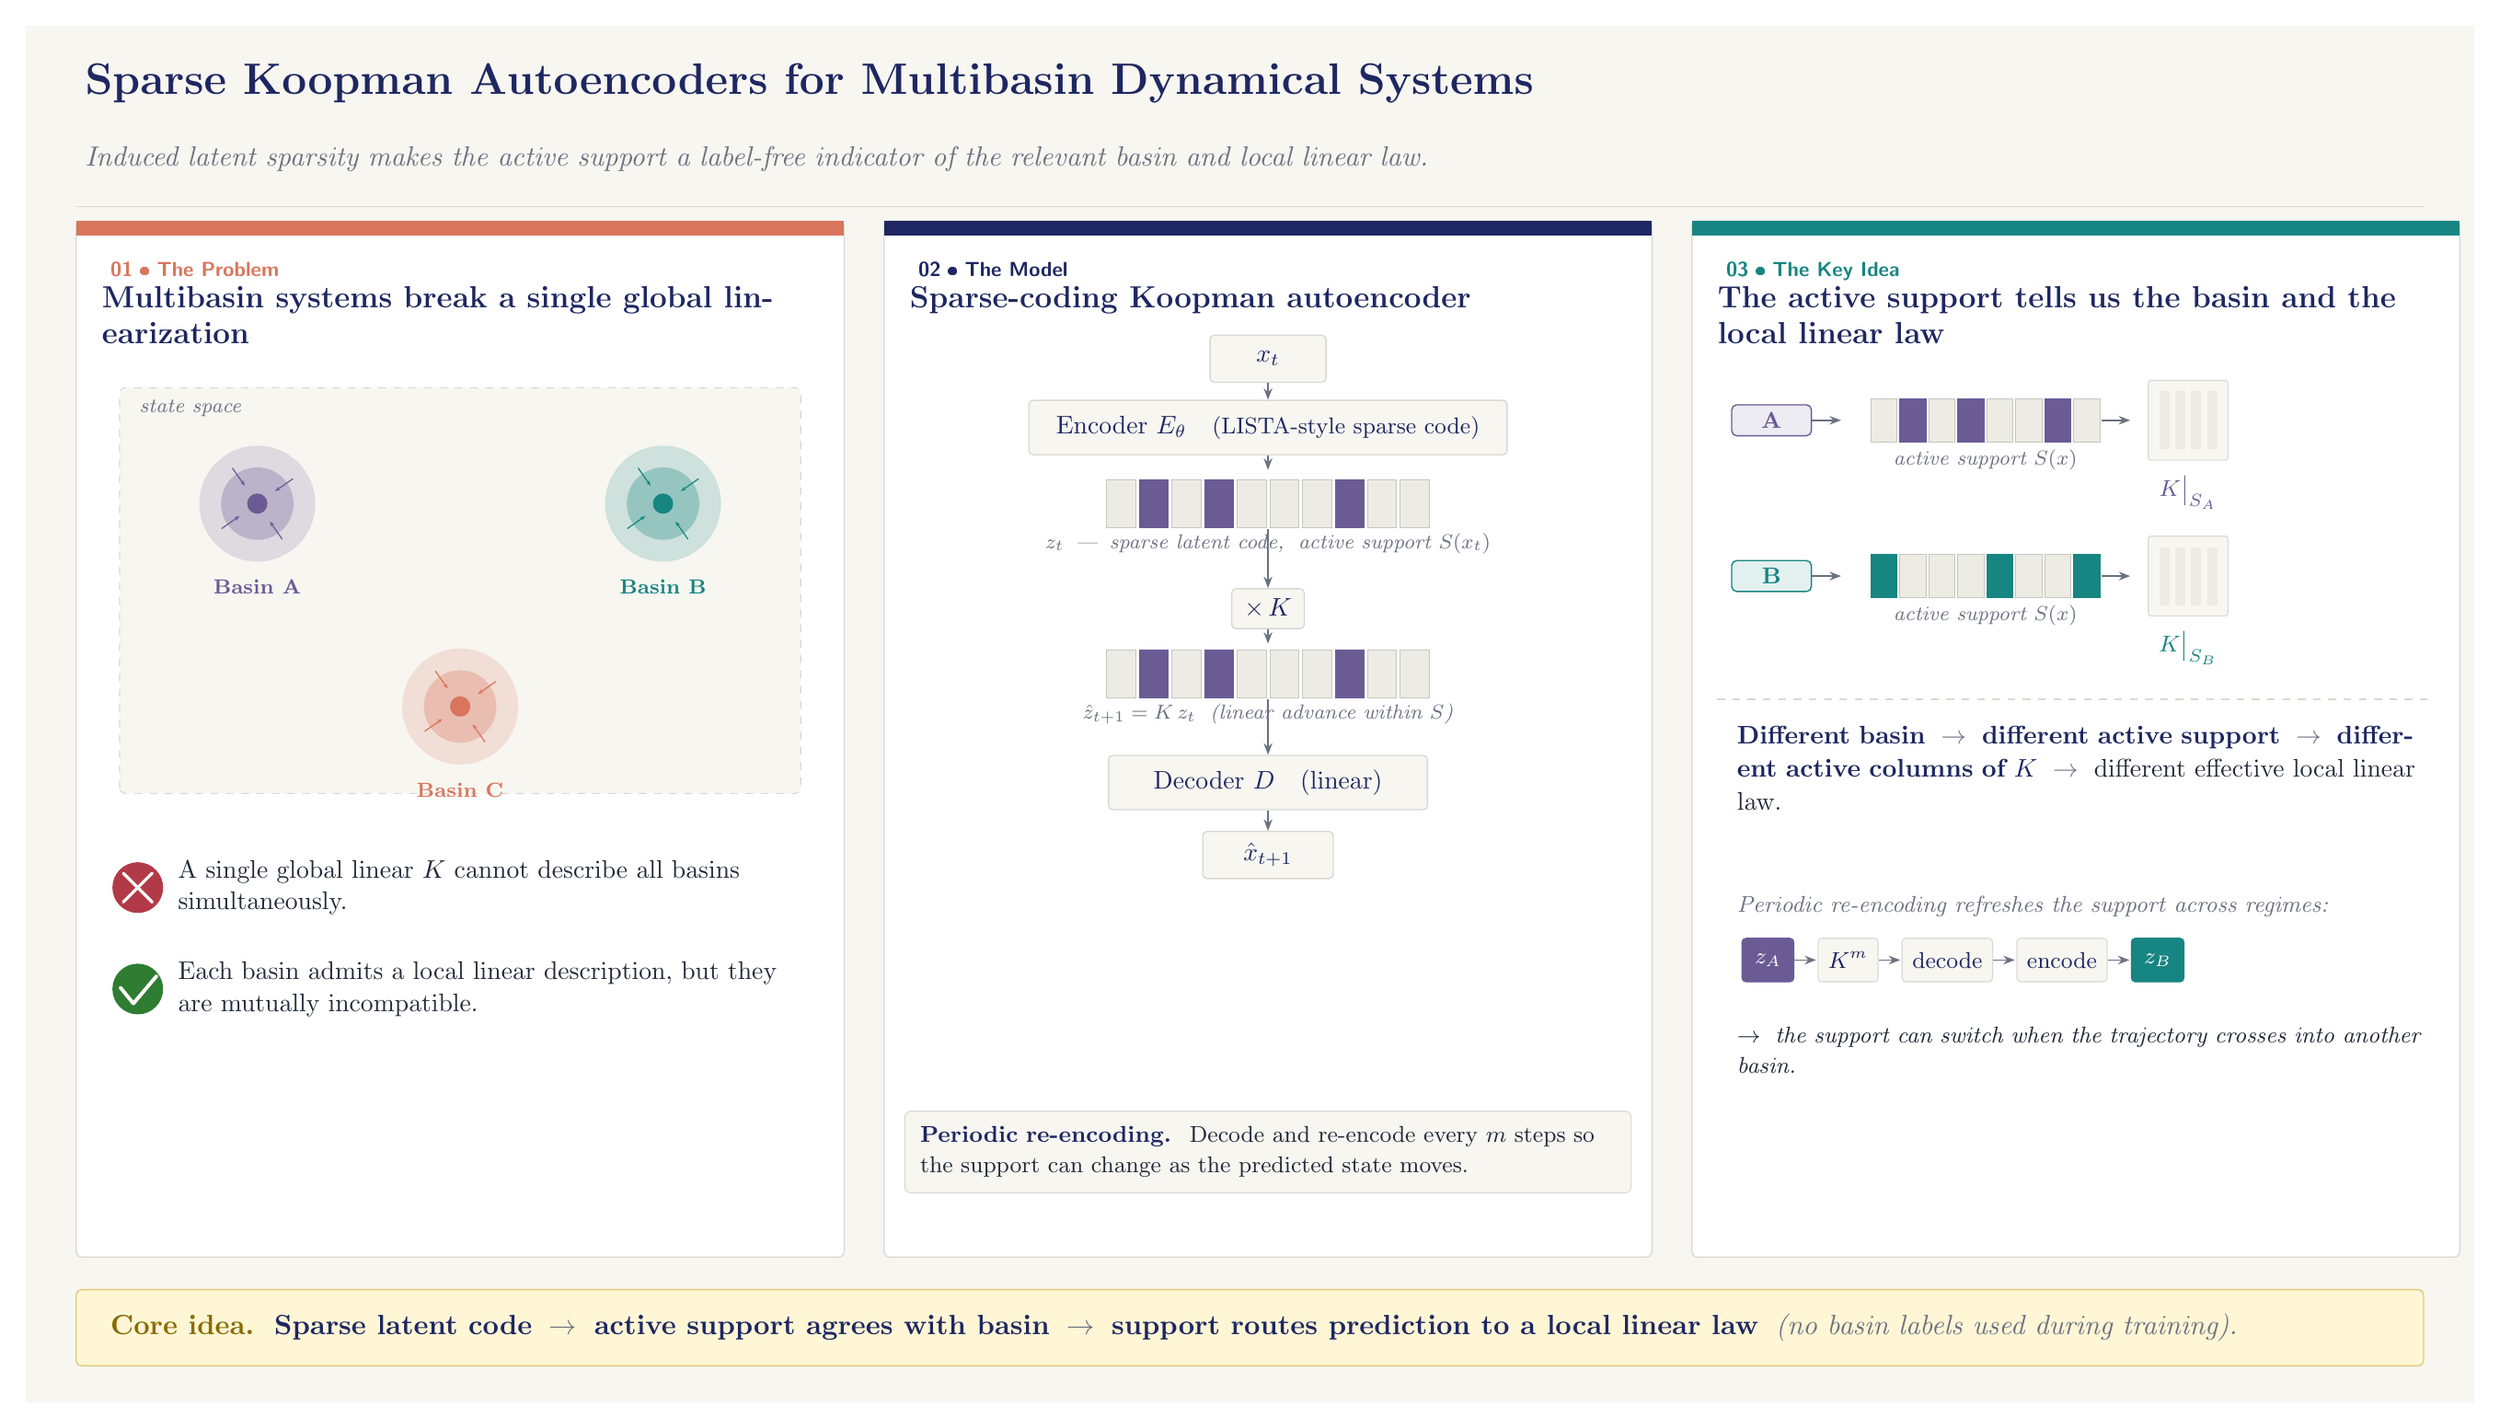
\begin{tikzpicture}[x=1cm,y=1cm,font=\rmfamily]

% =========================================================================
% Slide canvas — wide layout (33.8 x 19.0 cm ~= 13.3 x 7.5 in)
% =========================================================================
\fill[bgsoft] (0,0) rectangle (33.8,19);

% --- Title --------------------------------------------------------------
\node[anchor=north west,font=\fontsize{19}{22}\selectfont\bfseries,
      text=textdark]
  at (0.7,18.6)
  {Sparse Koopman Autoencoders for Multibasin Dynamical Systems};

\node[anchor=north west,font=\fontsize{11}{13}\selectfont\itshape,
      text=textmuted,text width=32cm]
  at (0.7,17.45)
  {Induced latent sparsity makes the active support a label-free indicator
   of the relevant basin and local linear law.};

\draw[cardborder,line width=0.4pt] (0.7,16.5) -- (33.1,16.5);

% =========================================================================
% Three panel cards — y range [2.0, 16.3], width 10.6 cm each, gap 0.55
% =========================================================================
% Panel A: x in [0.7, 11.3]
% Panel B: x in [11.85, 22.45]
% Panel C: x in [23.0, 33.6]
\foreach \xL/\acc in {0.7/basinC,11.85/textdark,23.0/basinB}{%
  \draw[draw=cardborder,line width=0.5pt,fill=cardbg,rounded corners=2pt]
    (\xL,2.0) rectangle ({\xL+10.6},16.3);
  \fill[\acc] (\xL,16.1) rectangle ({\xL+10.6},16.3);
}

% =========================================================================
% PANEL A — The Problem
% =========================================================================
\node[anchor=north west,paneltag=basinC]
  at (1.05,15.85) {01\;\textbullet\;\textsc{The Problem}};
\node[anchor=north west,paneltitle,text width=9.9cm]
  at (1.05,15.4)
  {Multibasin systems break a single global linearization};

% State-space sketch (rectangle 9.4cm x 6.0cm)
\draw[draw=cardborder,line width=0.4pt,dashed,fill=bgsoft,
      rounded corners=2pt]
  (1.3,8.4) rectangle (10.7,14.0);
\node[anchor=north west,font=\fontsize{8.5}{10}\selectfont\itshape,
      text=textmuted]
  at (1.45,13.95) {state space};

\drawbasin{3.2}{12.4}{basinA}{Basin~A}
\drawbasin{8.8}{12.4}{basinB}{Basin~B}
\drawbasin{6.0}{ 9.6}{basinC}{Basin~C}

% Two takeaways below scene
% bad row at y=7.0
\fill[badred] (1.55,7.10) circle (3.5mm);
\draw[white,line width=1.2pt,line cap=round]
  ($(1.55,7.10)+(-2.0mm,-2.0mm)$) -- ++(4mm,4mm);
\draw[white,line width=1.2pt,line cap=round]
  ($(1.55,7.10)+(-2.0mm,2.0mm)$) -- ++(4mm,-4mm);
\node[anchor=west,body,text width=8.3cm]
  at (2.1,7.10)
  {A single global linear $K$ cannot describe all basins simultaneously.};

% good row at y=5.6
\fill[okgreen] (1.55,5.7) circle (3.5mm);
\draw[white,line width=1.4pt,line cap=round,line join=round]
  ($(1.55,5.7)+(-2.4mm,0.2mm)$) --
  ($(1.55,5.7)+(-0.6mm,-2.0mm)$) --
  ($(1.55,5.7)+(2.6mm,1.8mm)$);
\node[anchor=west,body,text width=8.3cm]
  at (2.1,5.7)
  {Each basin admits a local linear description, but they are mutually
   incompatible.};

% =========================================================================
% PANEL B — The Model (vertical pipeline centered at x = 17.15)
% =========================================================================
\node[anchor=north west,paneltag=textdark]
  at (12.20,15.85) {02\;\textbullet\;\textsc{The Model}};
\node[anchor=north west,paneltitle,text width=9.9cm]
  at (12.20,15.4)
  {Sparse-coding Koopman autoencoder};

\def\bcx{17.15}

% x_t
\node[pipebox,minimum width=1.6cm,minimum height=0.65cm]
  (xt) at (\bcx,14.4) {$x_t$};

% Encoder
\node[pipebox,minimum width=6.6cm,minimum height=0.75cm]
  (enc) at (\bcx,13.45) {Encoder $E_\theta$\quad\small (LISTA-style sparse code)};

% z_t strip
\stripB{\bcx}{12.40}{{2,4,8}}{basinA}
\node[caption] at (\bcx,11.85)
  {$z_t$ \,---\, sparse latent code,\; active support $S(x_t)$};

% K arrow
\node[pipebox,minimum width=1.0cm,minimum height=0.55cm,
      font=\fontsize{10}{12}\selectfont\bfseries\itshape]
  (Kbox) at (\bcx,10.95) {$\times\,K$};

% zhat strip
\stripB{\bcx}{10.05}{{2,4,8}}{basinA}
\node[caption] at (\bcx,9.50)
  {$\hat{z}_{t+1}=K\,z_t$ \;(linear advance within $S$)};

% Decoder
\node[pipebox,minimum width=4.4cm,minimum height=0.75cm]
  (dec) at (\bcx,8.55) {Decoder $D$\quad(linear)};

% xhat
\node[pipebox,minimum width=1.8cm,minimum height=0.65cm]
  (xhat) at (\bcx,7.55) {$\hat{x}_{t+1}$};

% pipeline arrows
\draw[arr] (xt.south)  -- (enc.north);
\draw[arr] (enc.south) -- ++(0,-0.20);
\draw[arr] (\bcx,12.05) -- (Kbox.north);
\draw[arr] (Kbox.south) -- ++(0,-0.20);
\draw[arr] (\bcx,9.70)  -- (dec.north);
\draw[arr] (dec.south)  -- (xhat.north);

% Bottom callout
\node[draw=cardborder,line width=0.4pt,fill=bgsoft,
      rounded corners=2pt,inner sep=6pt,
      text width=9.6cm,align=left,
      font=\fontsize{9.5}{12}\selectfont,text=textbody]
  at (\bcx,3.45)
  {\textbf{\textcolor{textdark}{Periodic re-encoding.}}\;
   Decode and re-encode every $m$ steps so the support can change as the
   predicted state moves.};

% =========================================================================
% PANEL C — The Key Idea
% =========================================================================
\node[anchor=north west,paneltag=basinB]
  at (23.35,15.85) {03\;\textbullet\;\textsc{The Key Idea}};
\node[anchor=north west,paneltitle,text width=9.9cm]
  at (23.35,15.4)
  {The active support tells us the basin and the local linear law};

% --- Row 1 (Basin A) ---
\node[basinbadge=basinA] (bdA) at (24.10,13.55) {A};
\draw[arr] (bdA.east) -- ++(0.40,0);
\stripC{27.05}{13.55}{{2,4,7}}{basinA}
\node[caption] at (27.05,13.00) {active support $S(x)$};
\draw[arr] (28.65,13.55) -- ++(0.40,0);
\miniK{29.85}{13.55}{basinA}{{1,3}}
\node[font=\fontsize{9.5}{11}\selectfont\itshape,text=basinA]
  at (29.85,12.55) {$K\bigl|_{S_A}$};

% --- Row 2 (Basin B) ---
\node[basinbadge=basinB] (bdB) at (24.10,11.40) {B};
\draw[arr] (bdB.east) -- ++(0.40,0);
\stripC{27.05}{11.40}{{1,5,8}}{basinB}
\node[caption] at (27.05,10.85) {active support $S(x)$};
\draw[arr] (28.65,11.40) -- ++(0.40,0);
\miniK{29.85}{11.40}{basinB}{{2,4}}
\node[font=\fontsize{9.5}{11}\selectfont\itshape,text=basinB]
  at (29.85,10.40) {$K\bigl|_{S_B}$};

% --- Divider ---
\draw[cardborder,line width=0.4pt,dashed]
  (23.35,9.7) -- (33.25,9.7);

% --- Mechanism explanation ---
\node[anchor=north west,
      font=\fontsize{10}{13}\selectfont,
      text=textbody,align=left,text width=9.6cm]
  at (23.50,9.45)
  {\textbf{\textcolor{textdark}{Different basin}}
   {\color{textmuted}\;$\to$\;}
   \textbf{\textcolor{textdark}{different active support}}
   {\color{textmuted}\;$\to$\;}
   \textbf{\textcolor{textdark}{different active columns of $K$}}
   {\color{textmuted}\;$\to$\;}
   different effective local linear law.};

% --- Periodic re-encoding refresh ---
\node[anchor=north west,
      font=\fontsize{9.5}{11}\selectfont\itshape,text=textmuted]
  at (23.50,7.10)
  {Periodic re-encoding refreshes the support across regimes:};

% sequence
\node[seqcolor=basinA] (sa)   at (24.05,6.10) {$z_A$};
\draw[arr] (sa.east) -- ++(0.30,0);
\node[seqbox,right=0.32 of sa]   (km)  {$K^{m}$};
\draw[arr] (km.east) -- ++(0.30,0);
\node[seqbox,right=0.32 of km]   (de)  {decode};
\draw[arr] (de.east) -- ++(0.30,0);
\node[seqbox,right=0.32 of de]   (en)  {encode};
\draw[arr] (en.east) -- ++(0.30,0);
\node[seqcolor=basinB,right=0.32 of en] (sb) {$z_B$};

% bottom note
\node[anchor=north west,
      font=\fontsize{9.5}{12}\selectfont\itshape,text=textbody,
      align=left,text width=9.6cm]
  at (23.50,5.30)
  {$\to$\; the support can switch when the trajectory crosses into another
   basin.};

% =========================================================================
% Footer band — Core idea
% =========================================================================
\draw[draw=ideabd,line width=0.5pt,fill=ideabg,rounded corners=2pt]
  (0.7,0.50) rectangle (33.1,1.55);
\node[anchor=west,
      font=\fontsize{10.5}{13}\selectfont,
      text=textdark]
  at (1.05,1.025)
  {\textbf{\textcolor[HTML]{8A6C00}{Core idea.}}\;
   \textbf{Sparse latent code}
   {\color{textmuted}\;$\to$\;}
   \textbf{active support agrees with basin}
   {\color{textmuted}\;$\to$\;}
   \textbf{support routes prediction to a local linear law}\;
   \textit{\textcolor{textmuted}{(no basin labels used during training).}}};

\end{tikzpicture}
\end{document}
